\documentclass[10pt,table]{beamer}

% beamer theme
\usetheme{Boadilla}
\usefonttheme[onlymath]{serif}
\linespread{1.15}
\usepackage{parskip}
\setlength{\parskip}{6pt}
\usepackage{moresize}

\usepackage{etoolbox}

\newcounter{multipleslide}

\makeatletter%
\newcommand{\multipleframe}{%
	\setcounter{multipleslide}{\value{framenumber}}
	\stepcounter{multipleslide}
	\patchcmd{\beamer@@tmpl@footline}% <cmd>
	{\insertframenumber}% <search>
	{\themultipleslide}% <replace>
	{}% <success>
	{}% <failure>
}
\newcommand{\restoreframe}{%
	\patchcmd{\beamer@@tmpl@footline}% <cmd>
	{\themultipleslide}% <search>
	{\insertframenumber}% <replace>
	{}% <success>
	{}% <failure>
	\setcounter{framenumber}{\value{multipleslide}}%
}
\makeatother%


% language settings
\usepackage[utf8]{inputenc}
\usepackage[T1]{fontenc}
\usepackage[english]{babel} % English
\usepackage{kotex} % Korean
\usepackage{ulem} % underline environments
\usepackage[]{hyperref} % manage links, e.g. internal links, urls, etc.
\usepackage{wasysym} % hexagon, etc.


% include code
\usepackage{listings}
\lstset { %
	language=C++, % language
	backgroundcolor=\color{gray!5}, % set backgroundcolor
	tabsize=3, % tab spacing size
	breaklines=true, % enable linebreak
	postbreak=\mbox{\textcolor{red}{$\hookrightarrow$}\space},
	basicstyle=\color{green!40!black}\ssmall,
	keywordstyle=\bfseries\color{green!40!black},
	commentstyle=\itshape\color{red!80!black},
	identifierstyle=\color{blue},
	stringstyle=\color{purple!40!black},
	showstringspaces=false,
	numbers=left,
	stepnumber=1,
	xleftmargin=2em,
}


% arrays
\usepackage{array,multirow,multicol,tabularx} % tables
\newcolumntype{Y}{>{\centering\arraybackslash}X}
%\usepackage[table]{xcolor}

% graphics
%\usepackage{graphicx,caption,subcaption} % inclusion of graphics and captions
\usepackage{tikz} % TikZ
%\usepackage{pgfplots} % for functional plots in tikz environment
\usetikzlibrary{arrows} % arrow style
\usetikzlibrary{arrows.meta,bending}
\usetikzlibrary{calc}
\tikzset{>=latex}
\usetikzlibrary{patterns} % patterns used to fill the interior of regions, etc.
%\usetikzlibrary{hobby} % im­ple­ments Hobby’s al­go­rithm for a path built out of Bezier curves which passes through a given set of points, used for drawing plots that do not use a functional expression
\newcommand*\circled[1]{\tikz[baseline=(char.base)]{
		\node[shape=circle,draw,inner sep=2pt] (char) {#1};}}

% mathematics
\usepackage{amsmath,amssymb,mathtools}
\usepackage{cancel} % cancelation of terms
\usepackage{nicefrac} % certain fraction styles
\newcommand*{\diff}{\mathop{}\!\mathrm{d}} % differential



\title[FFT]{FFT and Applications}
\subtitle{Lecture ETC-2}
\author{Cheong-Eung Ahn}
\date{\today}

\begin{document}

\def\arraystretch{1.2}

\begin{frame}
\titlepage
\end{frame}

\begin{frame}{Definitions: Fourier Transform}
\textbf{Fourier transform (FT)} is the decomposition of a \textit{function of time}, $f\::\:\mathbb{R}\rightarrow\mathbb{C}$ to a \textit{function of frequency} with the \textbf{integral transform},
\begin{equation*}
\hat{f}(\xi)=\int_{-\infty}^\infty f(x)e^{-2\pi ix\xi}\diff x
\end{equation*}
Fourier transforms are extensively used in the solution of PDEs such as the heat equation (original development by Fourier), the wave equations of QM and QFT (Sch\"{o}rdinger equation, Klein-Gordon-Fock equation, etc.), signal processing, spectroscopic methods such as FTIR, etc.

\vfill

Examples:
\begin{figure}
\centering
\fbox{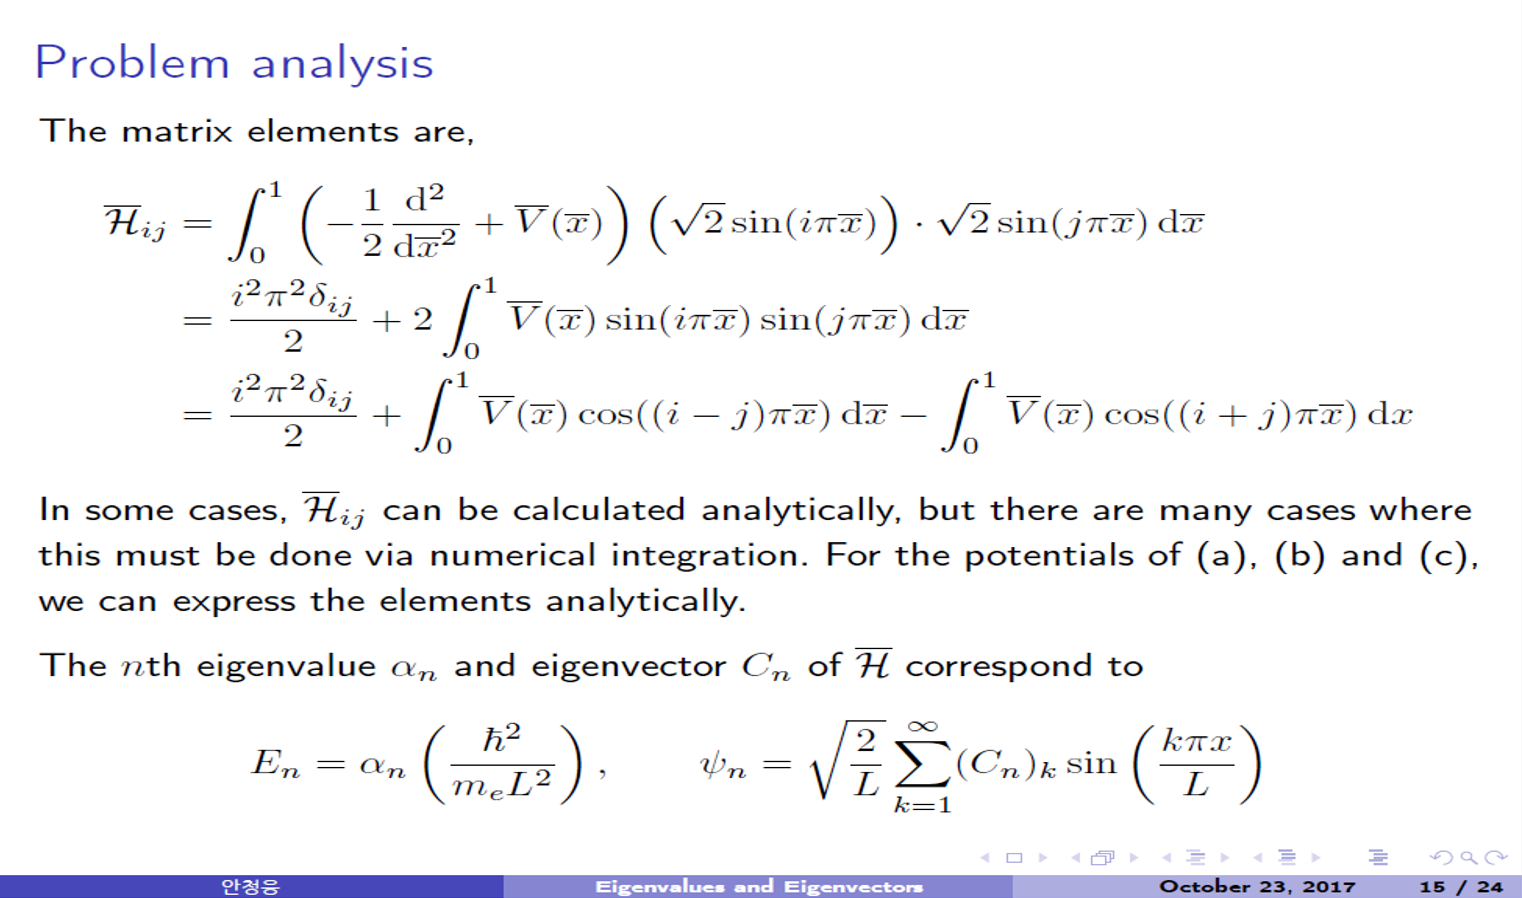
\includegraphics[height=0.18\linewidth]{FFT_ex1.png}}
\hspace{0.04\linewidth}
\fbox{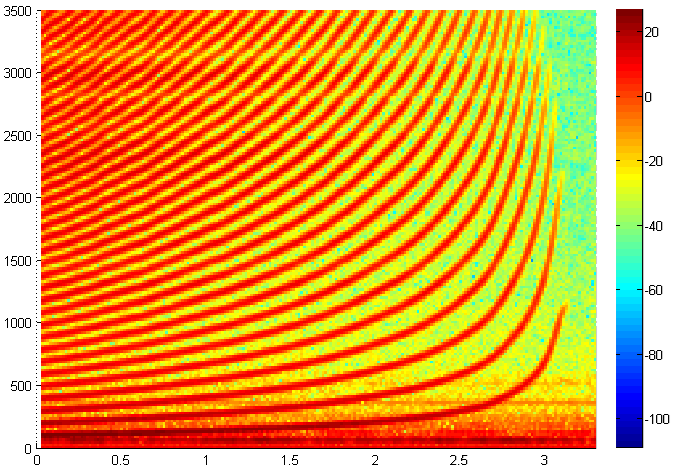
\includegraphics[height=0.18\linewidth]{FFT_ex2.png}}
\hspace{0.04\linewidth}
\fbox{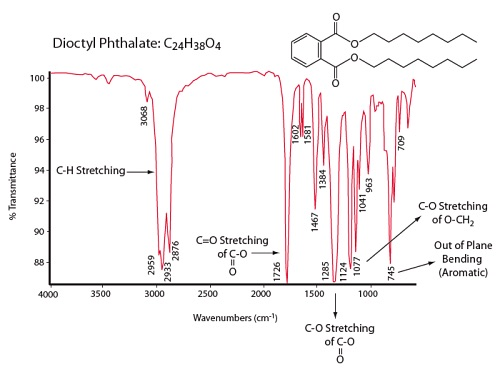
\includegraphics[height=0.18\linewidth]{FFT_ex3.jpg}}
\end{figure}
\end{frame}

\begin{frame}{Definitions: FFT}
\textbf{Fast Fourier transform (FFT)} is often used synonymously with FT in the context of signal processing. However, it actually refers to a specific class of algorithms which computes the \textbf{discrete Fourier transform (DFT)},
\begin{equation*}
\mathcal{F}\::\:X_k=\sum_{n=0}^{N-1}x_n\cdot e^{-i2\pi kn/N}=\sum_{n=0}^{N-1}x_n\left[\cos(2\pi kn/N)-i\cdot\sin(2\pi kn/N)\right]
\end{equation*}
The \textbf{inverse discrete Fourier transform (iDFT)} can be done as
\begin{equation*}
\mathcal{F}^{-1}\::\:x_n=\sum_{k=0}^{N-1}X_k\cdot e^{i2\pi nk/N}
\end{equation*}

\vfill

The main use of FFT in context of competitve programming arises in calculating the \textbf{convolution} of two sequences. The convolution theorem shows a \textbf{duality} between the DFT and convolution.
\end{frame}

\begin{frame}{Definitions: Convolution}
\begin{block}{The Polynomial Multiplication Problem}
Given two polynomials $A(x)$ and $B(x)$, calculate $C(x)=A(x)B(x)$.
\begin{gather*}
A(x)=\sum_{i=0}^{n-1}a_ix^i,\qquad B(x)=\sum_{i=0}^{n-1}b_ix^i\\
C(x)=\sum_{k=0}^{2n-2}c_kx^k\quad\text{such that}\quad c_k=\sum_{i=0}^{k}a_ib_{k-i}
\end{gather*}
\underline{Remark}: We use the extension that $a_i=b_i=0$ for $i<0$ and $i\geq n$.
\end{block}
ex) Big number multiplication, generating functions, etc.

The sequence $\{c_k\}$ is the \textbf{discrete convolution} of $\{a_i\}$ and $\{b_i\}$. Another important convolution is the \textbf{cyclical convolution} where $a_i$ for $i<0$ and $i\geq n$ are defined as the remainder modulo $n$ (hence the convention of $[n]$)\footnote{$[n]=\{0,1,...,n-1\}$}.
\end{frame}

\begin{frame}{Convolution Theorem}
The \textbf{convolution theorem} states that convolution in one domain equals pointwise multiplication in the other domain, i.e.
\begin{equation*}
\mathcal{F}\{f*g\}=\mathcal{F}\{f\}\cdot\mathcal{F}\{g\},\qquad\mathcal{F}\{f\cdot g\}=\mathcal{F}\{f\}*\mathcal{f}\{g\}
\end{equation*}
where $\cdot$ denotes pointwise multiplication (not polynomial multiplication). This works both for the discrete and cyclic convolutions. This theorem also holds for the inverse Fourier transform, Laplace transform, etc.

\vfill

Therefore, our strategy for solving the polynomial multiplication problem is
\begin{equation*}
C(x)=A(x)B(x)\qquad\longleftrightarrow\qquad\mathbf{c}=\mathbf{a}*\mathbf{b}=\mathcal{F}^{-1}\left\{\mathcal{F}\{\mathbf{a}\}\cdot\mathcal{F}\{\mathbf{b}\}\right\}
\end{equation*}
As pointwise multiplication requires only $\mathcal{O}(n)$ time, the complexity is dominated by the time required for FFT which is $\mathcal{O}(n\lg n)$.
\end{frame}

\begin{frame}{Primitive Roots of Unity in $\mathbb{C}$}
Despite most input and output variables in CP problems being integers, or at the very least real, we consider $\mathbb{Z}_+\rightarrow\mathbb{C}$ function to make use of the algebraic structure of $\mathbb{C}$.

For $\mathbb{C}$, we have the existence of \textbf{primitive roots of unity}, $\omega\in\mathbb{C}$ such that $\omega^N=1$ and $\omega^k\neq 1$ for $k\in[N]$. For example, $\omega=e^{-i2\pi/N}$.

\vfill

\begin{center}
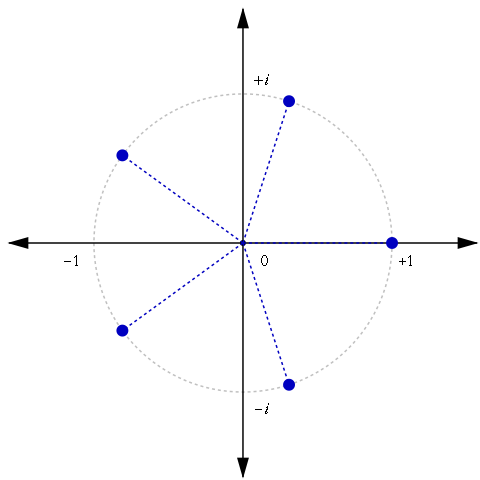
\includegraphics[width=0.36\linewidth]{roots.png}
\end{center}
\end{frame}

\begin{frame}{Divide and Conquer}
Rewriting the DFT in context of roots of unity,
\begin{equation*}
\mathcal{F}\::\:A_i=\sum_{j=0}^{N-1}a_j\omega^{ij}=a(\omega^i),\qquad\mathcal{F}^{-1}\::\:a_j=\sum_{i=0}^{N-1}A_i\omega^{-ij}=A(\omega^{-i})
\end{equation*}
where $a(x)=\sum a_kx^k$, $A(x)=\sum A_kx^k$. Trivially, we can calculate in $\mathcal{O}(n^2)$.

We consider the \textbf{radix-2 DIT Cooley–Tukey FFT algorithm} (most common implementation) which uses the \textit{divide and conquer} paradigm to optimize.

Let $N_0=2N_1$. We can divide a polynomial into even and odd terms.
\begin{equation*}
a_{0,0}(x)\qquad=\qquad\underbracket{\sum_{k=0}^{N_1-1}a_{2k}x^{2k}}_{=a_{1,0}(x^2)}\qquad+\qquad x\underbracket{\sum_{k=0}^{N_1-1}a_{2k+1}x^{2k}}_{=a_{1,1}(x^2)}
\end{equation*}
Assume we have the DFT of $\{a_{1,0}\}$ and $\{a_{1,1}\}$, $\{A_{1,0}\}$ and $\{A_{1,1}\}$ using the primitive root of unity $\omega_1=e^{-i2\pi/N_1}=\omega^2$.
\end{frame}

\begin{frame}{Divide and Conquer (cont.)}
Then for $0\leq i<N_1$,
\begin{equation*}
A_{0,0,i}=a_{0,0}(\omega_0^{i})=a_{1,0}(\omega_1^{i})+\omega_0^ia_{1,1}(\omega_1^{i})=A_{1,0,i}+\omega_0^iA_{1,1,i}
\end{equation*}
Similarly,
\begin{equation*}
A_{0,0,N_1+i}=A_{1,0,i}-\omega_0^iA_{1,1,i}
\end{equation*}
The factor $\omega_0^i$ is sometimes refered to as the twiddle factor.

Therefore, if we know $\{\{A_{1,v}\}_{v=0}^{2^1-1=1}\}$ we can find $\{\{A_{0,v}\}_{v=0}^{2^0-1=0}\}$ in $\mathcal{O}(n)$.

\vfill

Let us use $N=N_0=2^n$ and $N_p=2^{n-p}$. We can recursively calculate,
\begin{equation*}
\underbracket{\left\{\left\{A_{p,v,k}\right\}_{v=0}^{2^p-1}\right\}_{k=0}^{N_p-1}}_{2^p\times N^p=2^n=N}\qquad\underset{\mathcal{O}(N)}{\longleftarrow}\qquad\underbracket{\left\{\left\{A_{p+1,v,k}\right\}_{v=0}^{2^{p+1}-1}\right\}_{k=0}^{N_{p+1}-1}}_{2^{p+1}\times N^{p+1}=2^n=N}
\end{equation*}
Therefore, overall complexity is $\mathcal{O}(nN)=\mathcal{O}(N\lg N)$.
\end{frame}

\begin{frame}{FFT Implementation}
content...
\end{frame}

\begin{frame}{Primitive Roots of Unity in $\mathbb{Z}_p$ and NTT}
One problem with DFT is that floating point arithmetic accumulates in error. One way to avoid this problem is to use the \textbf{number theoretic transform (NTT)} which considers functions $\mathbb{Z}_+\rightarrow\mathbb{Z}_p$ not $\mathbb{Z}_+\rightarrow\mathbb{C}$. However, this is not advisable for contests without access to notes due to suitable $p$ being rare. For most cases, rounding will provide more than accurate results.

For $N=2^n$, DFT uses $\omega=e^{\pm i2\pi/N}$. For NTT modulo $p=a\times 2^b+1$, we use $\omega=(x^a)^{2^b/N}$ where $x$ is a primitive root of $p$. $\omega$ is a primitive root of unity following from FLT. We must use $p$ s.t. $b\geq n$.

Useful primes and root of unity:
\begin{table}
\begin{tabularx}{\linewidth}{Y|c|c|Y|Y}
Prime & $a$ & $b$ & Primitive root & Data type\\\hline
3,221,225,473 &  3 & 30 &  5 & 64bit unsigned\\
2,281,701,377 & 17 & 27 &  3 & 64bit signed\\
2,013,265,981 & 15 & 27 & 31 & 64bit signed\\
  469,762,049 &  7 & 26 &  3 & 64bit signed
\end{tabularx}
\end{table}
\end{frame}

\begin{frame}{NTT Implementation}
content...
\end{frame}

\begin{frame}{XOR Convolution}
content...
\end{frame}

\begin{frame}{Problems}
Problem set by \texttt{koosaga}. Will select some from here and additional.
\begin{itemize}
	\item \url{https://www.acmicpc.net/workbook/view/824}
	\item \url{http://codeforces.com/problemset/tags/fft}
\end{itemize}
\end{frame}

\begin{frame}{Summary}
\begin{itemize}
	\item The Fourier transform is the decomposition of a function (sequence) in one domain to another using primitive roots of unity.
	\item By the convolution theorem, convolution (quadratic time) in one domain becomes pointwise multiplication (linear time) in another.
	\item FFT algorithms compute the DFT in $\mathcal{O}(n\lg n)$ time. Most common is the Cooley-Tukey algorithm which uses the divide and conquer paradigm.
	\item FFT can be generalized to various other convolutions and transforms, notably the number theoretic transform (NTT) and XOR convolution.
	\item For some problems, we must find the right convolution and transform to calculate the desired queries. This makes FFT problems hard to recognize.
	\item It is best to understand FFT/NTT conceptually and make use of team notes for the implementation.
\end{itemize}
\end{frame}
\end{document}